\chapter{Approach}
\label{twotierapproach}
I propose a two-tier approach to our problem. In the first tier, it plays the role of a \textit{filter}, and attempts to filter out the General citations, leaving behind the Specific citations to be passed to the second tier. Figure \ref{fig:twotier} illustrates the flow of our approach.
\begin{figure}[h]
  \centering
  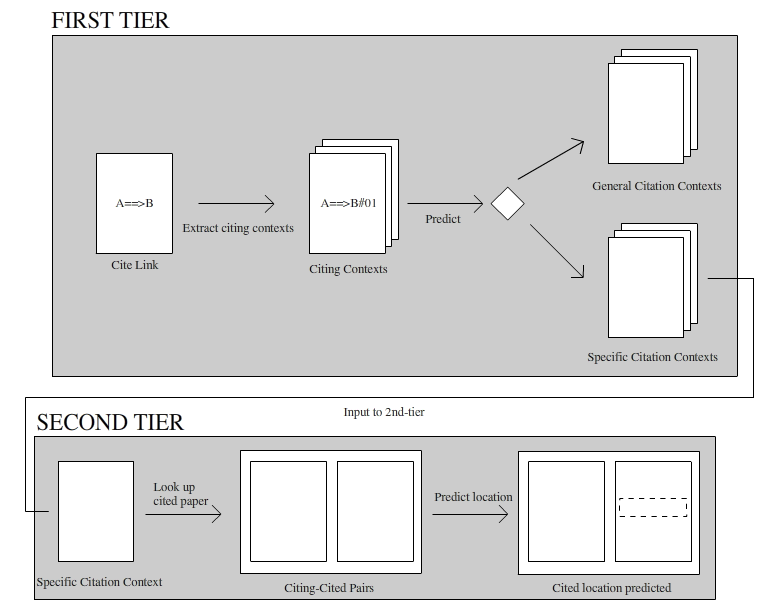
\includegraphics[scale=0.60]{./twotier}
  \caption{A Two-Tier Approach}
  \label{fig:twotier}
\end{figure}

\subsection{First Tier}
The First Tier is our attempt to filter out the General citations. In this tier, we are performing a 2-class \textit{citation classification} task, which already is a challenging task in the research area of citation analysis. We are not interested in determining whether the citation is one of the 12 class as defined by \cite{teufel2009annotation}, but only whether it is General or Specific. For each cite link we extract its citing contexts. Then for these contexts we extract feature vectors in order to pass it into our prediction model. We adopt similar features that were presented in previous works on citation classification.

\subsubsection{First Tier Features}
\begin{enumerate}
\item Physical Features \\
We adopted the physical features as presented in \cite{dongensemble}. They are:
\begin{enumerate}
\item \textit{Location}: in which section the citing sentence is from.
\item \textit{Popularity}: no. of citation marks in the citing sentence.
\item \textit{Density}: no. of unique citation marks in the citing sentence and its neighbour sentences.
\item \textit{AvgDens}: the average of Density among the citing and neighbour sentences.
\end{enumerate}

\item Number Density \\
A numerical feature that measures the density of numerical figures in the citing context. The intuition is that Specific citations tend refer to evaluation results in the cited paper. E.g. ``...Nivre and Scholz (2004) obtained a precision of 79.1\%...".

\item Publishing Year Difference \\
A numerical feature that represents difference in the publishing year between the citing and cited paper. The intuition is that higher difference suggests cited paper is older and presented a fundamental idea, and thus cited for General purposes.

\item Citing Context's Average \url{tf-idf} Weight \\
A numerical feature that indicates the amount of \textit{valuable} (as determined by \url{tf-idf} \cite{irtextbook}) words in the citing context. Higher values suggest important words and thus specific keywords.

\item Cue Words \\
Another numerical feature adopted from \cite{dongensemble}, that computes the amount of cue words (pre-defined manually by us) that appear in the citing sentence and its neighbour sentences. We defined 2 classes of cue words: Cue-General and Cue-Specific (refer to Appendix \ref{cuewords} for list of cue words). These cue words are selected based on the examples we observed in our training corpus.
\end{enumerate}
From our training corpus we extracted these features to build our First Tier Model for prediction.

\subsection{Second Tier}
In our Second Tier, it is another abstraction of our problem. It is independent from the First tier. We assume all the inputs into the second tier are Specific citations, and then we attempt to predict which of the fragments in the cited paper is the cited fragment.

\subsubsection{Second Tier Features}
\begin{enumerate}
\item Surface Matching \\
A numerical feature that measures the amount of word overlap between the citing sentence and a fragment in the cited paper.

\item Number Near-Miss \\
A numerical feature that measures the amount of numerical figures overlap between the citing sentence and a fragment in the cited paper. This feature will preprocess each fragment, rounding numerical figures or converting to percentage values, when it tries to match the numerical figures in the citing sentence. The intuition for this feature is from our observations that most Specific citations refer to evaluation results in the cited paper.

\item Bigrams Matching \\
A numerical feature that measures the amount of bigrams overlap between the citing sentence and a fragment in the cited paper. This feature is to preserve word order when comparing the citing sentence and the fragment. This feature is also targeted at Specific citations that refer to the cited paper for term definitions and quoting.

\item Cosine Similarity \\
A common numerical feature used in information retrieval tasks to measure similarity between the query and a candidate document. In our case, citing sentence and the fragment.
\end{enumerate}
Similarly we extracted these features from our training data to build our Second Tier Model for prediction.